\section{Exercise 3}
%-------------------------------------------------------------------------%
% Part a.                                                                 %
%-------------------------------------------------------------------------%
\subsection{Part a.}
Find the matrix that transforms a vector $(x_{1}, x_{2}, x_{3})$ into 
$(x_{2}, x_{3}, x_{1})$ in 3D. Verify that this is a rotation matrix and
give its axis and angle of rotation.
\begin{mdframed}[style=MyFrame]
    First we start by rotating the axes shown in Fig.~(\ref{fig:rotation}),
    which we can express in  matrix form as
    \begin{equation}
        R = 
        {\color{red}
        \begin{bmatrix}
            \cos 90^{\circ}     &   -\sin 90^{\circ}    &   0   \\
            \sin 90^{\circ}     &   \cos 90^{\circ}     &   0   \\
            0                   &   0                   &   1
        \end{bmatrix}
        }
        {\color{green}
        \begin{bmatrix}
            1                   &   0                   &   0                   \\
            0                   &   \cos 90^{\circ}     &   -\sin 90^{\circ}    \\
            0                   &   \sin 90^{\circ}     &   \cos 90^{\circ}     \\
        \end{bmatrix}
        }
    \end{equation}
    \begin{figure}[H]
        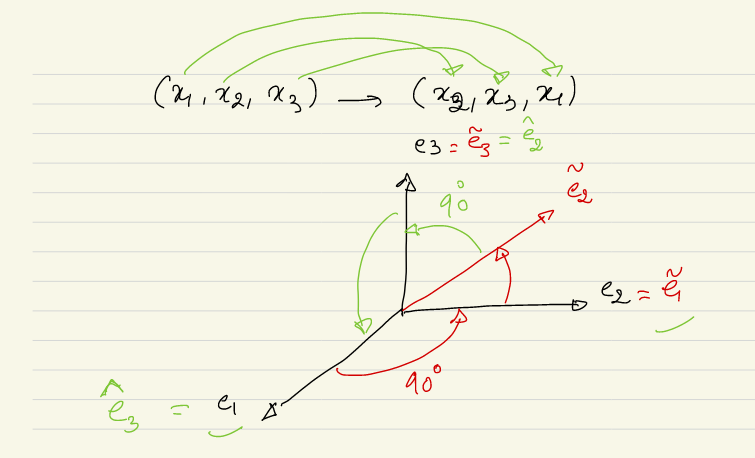
\includegraphics[height=0.35\textheight]{media/rotation.png}
        \caption{axes rotation}
        \label{fig:rotation}
    \end{figure}
    Therefore,
    \begin{equation}
        R =
        \begin{bmatrix}
            0       &       0       &       1       \\
            1       &       0       &       0       \\
            0       &       1       &       0
        \end{bmatrix}
    \end{equation}
    Next we can verify that $R$ is a rotational matrix with 
    \begin{equation}
        R
        \begin{bmatrix}
            x_{2}   \\
            x_{3}   \\
            x_{1}
        \end{bmatrix}
        =
        \begin{bmatrix}
            x_{1}   \\
            x_{2}   \\
            x_{3}
        \end{bmatrix}
    \end{equation}
    and
    \begin{equation}
        \begin{bmatrix}
            x_{2}   \\
            x_{3}   \\
            x_{1}
        \end{bmatrix}
        =
        R^{T}
        \begin{bmatrix}
            x_{1}   \\
            x_{2}   \\
            x_{3}
        \end{bmatrix}
    \end{equation}
    Therefore since $R$ is orthogonal and $R^{T}=R^{-1}$ verifies that $R$
    is a rotational matrix. Next we can find the axis of rotation $a$ using 
    $Ra=a \rightarrow (R-I)a = 0$, therefore the axis of rotation is the
    basis of the nullspace of $R-I$. We can find the basis of the nullspace
    from the row reduced echelon form
    \begin{equation}
        \text{rref}(R-I) =
        \begin{bmatrix}
            1   &   0   &   -1  \\
            0   &   1   &   -1  \\
            0   &   0   &   0
        \end{bmatrix}
    \end{equation}
    Thus,
    \begin{equation}
        a =
        \begin{bmatrix}
            1   \\
            1   \\
            1
        \end{bmatrix}
    \end{equation}
    Lastly, the angle of rotation can be found from the scalar product,
    namely
    \begin{equation}
        \mathbf{x}^{T}R\mathbf{x} = \norm{\mathbf{x}} \norm{R\mathbf{x}}\cos \theta
    \end{equation}
    \begin{equation}
        \cos \theta =
                        \frac{\mathbf{x}^{T}R\mathbf{x}}
                                {\norm{x}\norm{x}}
    \end{equation}
    where $\mathbf{x}$ is any vector that satisfies $\mathbf{x}^{T}a=0$.
    Setting
    \begin{equation}
        \mathbf{x} =
        \begin{bmatrix}
            1   \\
            -2   \\
            1
        \end{bmatrix}
    \end{equation}
    and solving for $\theta$ we can determine the axis of rotation,
    \begin{equation}
        \theta  =
                \cos^{-1}
                    \left(\frac{\mathbf{x}^{T}R\mathbf{x}}{\norm{\mathbf{x}}\norm{\mathbf{x}}}\right)
                    =
                    \cos^{-1}\left( -\frac{3}{6}\right)
    \end{equation}
    Thus,
    \begin{equation}
        \theta = 120^{\circ}
    \end{equation}
    \begin{figure}[H]
        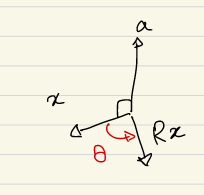
\includegraphics[height=0.35\textheight]{media/angle.png}
        \caption{Angle of rotation}
        \label{fig:angle}
    \end{figure}

\end{mdframed}
%-------------------------------------------------------------------------%
% Part b.                                                                 %
%-------------------------------------------------------------------------%
\subsection{Part b.}
Find the orthonormal vector $\mathbf{q}_{1}$, $\mathbf{q}_{2}$, and 
$\mathbf{q}_{3}$ such that $\mathbf{q}_{1}$ and $\mathbf{q}_{2}$ span the
column space of $\mathbf{A}$.
\begin{equation}
    \mathbf{A} =
    \begin{bmatrix}
        1       &       1       \\
        2       &       -1      \\
        -2      &       4       
    \end{bmatrix}
\end{equation}
\begin{enumerate}[label=(\arabic*)]
    \item Which of the four fundamental subspaces contain $\mathbf{q}_{3}$?
    \item Solve $\mathbf{A}\mathbf{x} = (4,5,2)$ by least squares?
\end{enumerate}
\begin{mdframed}[style=MyFrame]
    We can start by finding two orthonormal vectors $\mathbf{q}_{1}$ and
    $\mathbf{q}_{2}$ that span the column space,
    \begin{equation}
        \mathbf{q}_{1} =  \frac{\mathbf{v}_{1}}{\norm{\mathbf{v}_{1}}}
        \label{eq:part-b-q1}
    \end{equation}
    \begin{equation}
        \mathbf{q}_{2} =  \frac{\mathbf{v}_{2}}{\norm{\mathbf{v}_{2}}}
        \label{eq:part-b-q2}
    \end{equation}
    where,
    \begin{equation}
        \mathbf{v}_{1} = \mathbf{a}_{1} =  
        \begin{bmatrix}
            1   \\
            2   \\
            -2
        \end{bmatrix}
    \end{equation}
    and 
    \begin{equation}
        \mathbf{v}_{2} = 
        \mathbf{a}_{2} 
        - \frac{\mathbf{v}_{1}^{T} - \mathbf{a}_{2}}
            {\mathbf{v}_{1}^{T}\mathbf{v}_{1}}\mathbf{v}_{1}=  
        \begin{bmatrix}
            2   \\
            1   \\
            2
        \end{bmatrix}
    \end{equation}
    Substituting $\mathbf{v}_{1}$ and $\mathbf{v}_{2}$ into
    Eqs.~(\ref{eq:part-b-q1} \& \ref{eq:part-b-q2}), respectively, gives
    \begin{equation}
        \mathbf{q}_{1} = 
        \frac{1}{3}
        \begin{bmatrix}
            1       \\
            2       \\
            -2
        \end{bmatrix}
    \end{equation}
    and 
    \begin{equation}
        \mathbf{q}_{2} =
        \frac{1}{3}
        \begin{bmatrix}
            2       \\
            1       \\
            2
        \end{bmatrix}
    \end{equation}
    \newcommand{\qvec}[1]{\mathbf{q}_{#1}}
    Next, we can define $\qvec{3}$ as
    \begin{equation}
        \qvec{3} =
        \begin{bmatrix}
            a       \\
            b       \\
            c
        \end{bmatrix}
    \end{equation}
    and use the following relationships to determine $a$, $b$, and $c$,
    \begin{equation}
        \qvec{1}^{T}\qvec{3} = 0 \rightarrow
                \frac{1}{3} (a + 2b -2c) = 0
    \end{equation}
    \begin{equation}
        \qvec{2}^{T}\qvec{3} = 0 \rightarrow
                \frac{1}{3} (2a + b + 2c) = 0
    \end{equation}
    \begin{equation}
        \norm{\qvec{3}} = 1 \rightarrow a^{2} + b^{2} + c^{2} = 1
    \end{equation}
    Solving the first two equations in terms of $c$ we get
    \begin{equation}
        a = -2c
    \end{equation}
    and 
    \begin{equation}
        b = 2c
    \end{equation}
    Therefore,
    \begin{equation}
        4c^{2} + 4c^{2} + c^{2} = 1
    \end{equation}
    Thus, 
    \begin{equation}
        c = \pm \frac{1}{3}
    \end{equation}
    and 
    \begin{equation}
        \qvec{3} =
        \pm
        \frac{1}{3}
        \begin{bmatrix}
            -2      \\
            2       \\
            1
        \end{bmatrix}
    \end{equation}
    Lastly, since $\qvec{1}$ and $\qvec{2}$ span the column space and
    $\qvec{3}$ is perpendicular to them implies that $\qvec{3}$ is the left
    null space.
\end{mdframed}
%-------------------------------------------------------------------------%
% Part c.                                                                 %
%-------------------------------------------------------------------------%
\subsection{Part c.}
Find an orthonormal basis for the column space of $\mathbf{A}$ and compute
the projection of $\mathbf{b}$ onto that column space:
\begin{equation}
    \mathbf{A} =
    \begin{bmatrix}
        1       &       -2  \\
        1       &       0   \\
        1       &       1   \\
        4       &       2   \\
    \end{bmatrix}
\end{equation}
\begin{mdframed}[style=MyFrame]
    We start with by first finding orthonormal vectors that span the column
    space $\mathbf{q}_{1}$ and $\mathbf{q}_{2}$ using
    \begin{equation}
        \mathbf{q}_{1} =
            \frac{\mathbf{v}_{1}}{\norm{\mathbf{v}_{1}}}
    \end{equation}
    and 
    \begin{equation}
        \mathbf{q}_{2} =
            \frac{\mathbf{v}_{2}}{\norm{\mathbf{v}_{2}}}
    \end{equation}
    Where the direction vectors are found from the Gram-Schmidt process, namely
    \begin{equation}
        \mathbf{v}_{1} = \mathbf{x}_{1} = 
        \begin{bmatrix}
            1       \\
            1       \\
            1       \\
            1
        \end{bmatrix}
    \end{equation}
    \begin{equation}
        \mathbf{v}_{2} = 
                \mathbf{x}_{2} 
                - \frac{\mathbf{x}_{1}^{T}\mathbf{x}_{2}}
                {\mathbf{x}_{1}^{T} \mathbf{x}_{1}}
                \mathbf{x}_{1}
                =
                \begin{bmatrix}
                    -5/2        \\
                    -1/2        \\
                    1/2         \\
                    5/2
                \end{bmatrix}
    \end{equation}
    Therefore,
        \begin{equation}
            \mathbf{q}_{1} = 
            \frac{1}{2}
            \begin{bmatrix}
                1       \\
                1       \\
                1       \\
                1       
            \end{bmatrix}
        \end{equation}
        and 
        \begin{equation}
            \mathbf{q}_{2} = 
            \frac{1}{\sqrt{13}}
            \begin{bmatrix}
                -5/2    \\
                -1/2    \\
                1/2     \\
                5/2       
            \end{bmatrix}
        \end{equation}
    Next we can find the perpendicular direction of basis using,
        \begin{equation}
            \mathbf{p}  = \left( \mathbf{q}_{1}^{T} \mathbf{b} \right) \mathbf{q}_{1}
                            + \left( \mathbf{q}_{2}^{T} \mathbf{b} \right) \mathbf{q}_{2}
        \end{equation} 
        Last, we can subtract the projection of $\mathbf{b}$ along the basis leaving
        the perpendicular part. Thus
        \begin{equation}
            \mathbf{b} - \mathbf{p} = 
                \frac{1}{2}
                \begin{bmatrix}
                    -1      \\
                    -3      \\
                    7       \\
                    -3
                \end{bmatrix}
        \end{equation}
\end{mdframed}

%-------------------------------------------------------------------------%
% Part d.                                                                 %
%-------------------------------------------------------------------------%
\subsection{Part d.}
Find orthogonal vectors $\mathbf{A}$, $\mathbf{B}$, and $\mathbf{C}$ by
Gram-Schmidt from
\begin{equation}
    a = 
    \begin{bmatrix}
        1       \\
        1       \\
        2
    \end{bmatrix}
    \text{ and }
    b = 
    \begin{bmatrix}
        1       \\
        -1      \\
        0
    \end{bmatrix}
    \text{ and }
    c = 
    \begin{bmatrix}
        1       \\
        0       \\
        4
    \end{bmatrix}
\end{equation}
\begin{mdframed}[style=MyFrame]
    Begin by choosing $\mathbf{A}=\mathbf{a}$. Next, start with
    $\mathbf{b}$ and subtract its projection along $\mathbf{A}$ using 
    \begin{equation}
        \mathbf{B} =  \mathbf{b} 
                        - \frac{\mathbf{A}^{T} \mathbf{b} }
                                {\mathbf{A}^{T} \mathbf{A}}
                                \mathbf{A}
    \end{equation}
    which gives
    \begin{equation}
        \mathbf{B} = 
        \begin{bmatrix}
            1       \\
            -1      \\
            0
        \end{bmatrix}
        -
        \frac{0}{6}
        \begin{bmatrix}
            1       \\
            1       \\
            2
        \end{bmatrix}
        =
        \begin{bmatrix}
            1       \\
            -1      \\
            0
        \end{bmatrix}
    \end{equation}
    Continuing we can perform the next Gram-Schmidt step by subtracting off
    the projections of $\mathbf{c}$ from $\mathbf{A}$ and $\mathbf{B}$,
    using
    \begin{equation}
        \mathbf{C} =  \mathbf{c} 
                        - \frac{\mathbf{A}^{T} \mathbf{c} }
                                {\mathbf{A}^{T} \mathbf{A}}
                                \mathbf{A}
                        - \frac{\mathbf{B}^{T} \mathbf{c} }
                                {\mathbf{B}^{T} \mathbf{B}}
                                \mathbf{B}
    \end{equation}
    giving
    \begin{equation}
        \mathbf{C} = 
        \begin{bmatrix}
            1       \\
            0       \\
            4
        \end{bmatrix}
        -
        \frac{9}{6}
        \begin{bmatrix}
            1       \\
            1       \\
            2
        \end{bmatrix}
        -
        \frac{1}{2}
        \begin{bmatrix}
            1       \\
            -1      \\
            0
        \end{bmatrix}
        =
        \begin{bmatrix}
            -1      \\
            -1      \\
            1
        \end{bmatrix}
    \end{equation}
    Lastly we can normalize the vectors by dividing by their magnitudes,
    \begin{equation}
        \frac{\mathbf{A}}{\norm{\mathbf{A}}} =
            \frac{1}{\sqrt{6}}
            \begin{bmatrix}
                1       \\
                1       \\
                2
            \end{bmatrix}
    \end{equation}
    \begin{equation}
        \frac{\mathbf{B}}{\norm{\mathbf{B}}} =
            \frac{1}{\sqrt{2}}
            \begin{bmatrix}
                1       \\
                -1      \\
                0
            \end{bmatrix}
    \end{equation}
    \begin{equation}
        \frac{\mathbf{C}}{\norm{\mathbf{C}}} =
            \frac{1}{\sqrt{3}}
            \begin{bmatrix}
                -1      \\
                -1      \\
                1
            \end{bmatrix}
    \end{equation}
\end{mdframed}
%-------------------------------------------------------------------------%
% Part e.                                                                 %
%-------------------------------------------------------------------------%
\subsection{Part e.}
Find $\mathbf{q}_{1}$, $\mathbf{q}_{2}$, and $\mathbf{q}_{3}$ (orthonormal)
as combination of $\mathbf{a}$, $\mathbf{b}$, and $\mathbf{c}$ (independent
columns). Then write $\mathbf{A}$ as $\mathbf{QR}$.
\begin{equation}
    \mathbf{A} =
    \begin{bmatrix}
        1       &       2       &   4   \\
        0       &       0       &   5   \\
        0       &       3       &   6
    \end{bmatrix}
\end{equation}

\begin{mdframed}[style=MyFrame]
    We start by finding $\mathbf{q}_{1}$, $\mathbf{q}_{2}$, and
    $\mathbf{q}_{3}$ using
    \begin{equation}
        \mathbf{q}_{1} = \frac{A}{\norm{A}}
    \end{equation}
    \begin{equation}
        \mathbf{q}_{2} = \frac{B}{\norm{B}}
    \end{equation}
    \begin{equation}
        \mathbf{q}_{3} = \frac{C}{\norm{C}}
    \end{equation}
    where $\mathbf{A}$, $\mathbf{B}$, and $\mathbf{C}$ are found from the
    Gram-Schmidt process, namely
    \begin{equation}
        \mathbf{A} = \mathbf{a} = 
        \begin{bmatrix}
            1   \\
            0   \\
            0   \\
        \end{bmatrix}
    \end{equation}
    \begin{equation}
        \mathbf{B} = 
        \mathbf{\mathbf{b}} 
        - \frac{ \mathbf{A}^{T} \mathbf{b} }{ \mathbf{A}^{T}\mathbf{A} }\mathbf{A}
        =
        \begin{bmatrix}
            0   \\
            0   \\
            3   \\
        \end{bmatrix}
    \end{equation}
    \begin{equation}
        \mathbf{C} = 
        \mathbf{c} 
        - \frac{ \mathbf{A}^{T} \mathbf{c} }{ \mathbf{A}^{T}\mathbf{A} }\mathbf{A}
        - \frac{ \mathbf{B}^{T} \mathbf{c} }{ \mathbf{B}^{T}\mathbf{B} }\mathbf{B}
        =
        \begin{bmatrix}
            0   \\
            5   \\
            0   \\
        \end{bmatrix}
    \end{equation}
    Therefore,
    \begin{equation}
        \mathbf{q}_{1} =  
        \begin{bmatrix}
            1   \\
            0   \\
            0
        \end{bmatrix}
    \end{equation}
    \begin{equation}
        \mathbf{q}_{2} =  
        \begin{bmatrix}
            0   \\
            0   \\
            1
        \end{bmatrix}
    \end{equation}
    \begin{equation}
        \mathbf{q}_{3} =  
        \begin{bmatrix}
            0   \\
            1   \\
            0
        \end{bmatrix}
    \end{equation}
    Lastly we can find $\mathbf{R}$ using,
    \begin{equation}
        \mathbf{R} =
        \begin{bmatrix}
            \mathbf{q}_{1}^{T}\mathbf{a}    &   \mathbf{q}_{1}^{T}\mathbf{b}    &   \mathbf{q}_{1}^{T}  \mathbf{c}  \\
            0                               &   \mathbf{q}_{2}^{T}\mathbf{b}    &   \mathbf{q}_{2}^{T}  \mathbf{c}  \\
            0                               &   0                               &   \mathbf{q}_{3}^{T}  \mathbf{c}  \\
        \end{bmatrix}
    \end{equation}
    Thus,
    \begin{equation}
        \begin{bmatrix}
            \mathbf{a}      &       \mathbf{b}      &   \mathbf{c}  
        \end{bmatrix}
        = 
        \begin{bmatrix}
            \mathbf{q}_{1}  &       \mathbf{q}_{2}  &   \mathbf{q}_{3}  
        \end{bmatrix}
        \begin{bmatrix}
            \mathbf{q}_{1}^{T}\mathbf{a}    &   \mathbf{q}_{1}^{T}\mathbf{b}    &   \mathbf{q}_{1}^{T}  \mathbf{c}  \\
            0                               &   \mathbf{q}_{2}^{T}\mathbf{b}    &   \mathbf{q}_{2}^{T}  \mathbf{c}  \\
            0                               &   0                               &   \mathbf{q}_{3}^{T}  \mathbf{c}  \\
        \end{bmatrix}
        =
        \underbrace{
            \begin{bmatrix}
                1   &   0   &   0   \\
                0   &   0   &   1   \\
                0   &   1   &   0   \\
            \end{bmatrix}
        }_{=Q}
        \underbrace{
            \begin{bmatrix}
                1   &   2   &   4   \\
                0   &   3   &   6   \\
                0   &   0   &   5   \\
            \end{bmatrix}
        }_{=R}
    \end{equation}
\end{mdframed}
